%%Andreas Neubauer, May 2016
\documentclass[12pt,a4paper]{article}
\usepackage{graphicx}
\usepackage[utf8]{inputenc}
\usepackage[T1]{fontenc}
\usepackage{algpseudocode}
\usepackage{algorithm}
\usepackage{algorithmicx}
\usepackage{graphicx}
\usepackage{url}
\usepackage[paper=a4paper]{geometry}
\usepackage{subcaption}
\usepackage{tocbibind}

\graphicspath{{../figures/}}
\newcommand*\Let[2]{\State #1 $\gets$ #2}

\newtheorem{ex}{Example}
\textwidth 16.7cm
\textheight 25cm
\topmargin -2.7cm
\oddsidemargin 0.25cm
\parindent 0pt
\pagestyle{empty}
\begin{document}
 %BEGIN_FOLD
%
% -------- only change entries beginning here ----------------------------
%
% choose language of coverpage: german or english
\newif\ifeng
\engtrue
%\engfalse
%
%
% enter the title of the thesis
%
\def\title{Local Search for Renamable Horn}
%
%
% choose type of work: 0 ... Dissertation
%                      1 ... Diplomarbeit
%                      2 ... Masterarbeit
\def\type{3}
%
%
% enter name of degree, see examples below (as stated in your curriculum)
%
\def\degree{Bachelor of Science}
% e.g. Masterstudium
%\def\degree{Diplom-Ingenieur}
%\def\degree{Diplom-Ingenieurin}
%\def\degree{Master of Science}
%
% e.g. Diplomstudium Lehramt
%\def\degree{Magister der Naturwissenschaften}
%\def\degree{Magistra der Naturwissenschaften}
%
% e.g. Doktorratsstudium
%\def\degree{Doktor der technischen Wissenschaften}
%\def\degree{Doktorin der technischen Wissenschaften}
%\def\degree{Doktor der Naturwissenschaften}
%\def\degree{Doktorin der Naturwissenschaften}
%
%
% enter the study (Studienrichtung, as stated in your curriculum)
%
\def\study{Informatik}
% e.g. Diplomstudium:
%\def\study{Lehramt Mathematik}
%
% e.g. Masterstudium:
%\def\study{Industriemathematik}
%
% e.g. Doktorratsstudium
%\def\study{Technische Wissenschaften}
%\def\study{Naturwissenschaften}
%
%
% If the names for the following entries are too long, break them into several
% lines using \\
%
%
% enter the name of the student
%
\def\name{Schobesberger Christoph}
%
%
% enter the name of the institute (use translation for english version)
% e.g.
%\def\institute{Industrial Mathematics\\ Institute}
%\def\institute{Institut f\"ur\\ Industriemathematik}
%
\def\institute{Institute for Formal Models and Verification}
%
%
% enter the name of the supervisor and first thesis examiner
% only for type 0 (Dissertation) you need a second thesis examiner
% 
% for the german version you also have to enter the sex (male or female)
% of the supervisor/examiners
%
\def\supervisor{Armin Biere}
\newif\ifsupvismale
\supvismaletrue
%\supvismalefalse
%
%\def\secondexaminer{Name of 2. examiner}
\newif\ifsecexmale
\secexmaletrue
%\secexmalefalse
%
%
% if there has been assistance by a further person uncomment the following line
% and enter the name.
%
%\def\assist{Name of assistant}
%
%
% enter month year
% (the month when you brought it to the Prüfungs- und Anerkennungsservice)
%
\def\date{May 2020}
%
% do not change anything below this line
% -------------------------------------------------------------------------------
%
\def\ifundefined#1{\expandafter\ifx\csname#1\endcsname\relax}
\DeclareFontShape{OT1}{cmss}{m}{n}
  {<5><6><7><8><9><10><10.95><12><14.4><17.28><20.74><24.88><29.86><35.83>%
   <42.99><51.59><67><77.38>cmss10}{}
\DeclareFontShape{OT1}{cmss}{bx}{n}
  {<5><6><7><8><9><10><10.95><12><14.4><17.28><20.74><24.88><29.86><35.83>%
   <42.99><51.59><67><77.38>cmssbx10}{}
\makeatletter
\def\Huge{\@setfontsize\Huge{29.86pt}{36}}
\makeatother
%
\unitlength 1cm
\sffamily
\begin{picture}(16.7,0)

\ifeng
 \put(11.5,-2.5){\includegraphics[width=5.2cm]{jku_en}}
\else
 \put(11.5,-2.5){\includegraphics[width=5.2cm]{jku_de}}
\fi
\put(12.9,-4.2){\begin{minipage}[t]{3.9cm}\footnotesize%
\ifeng
 Submitted by\\
\else
 Eingereicht von\\
\fi
{\bfseries\name}%
\vskip 4mm%
\ifeng
 Submitted at\\
\else
 Angefertigt am\\
\fi
{\bfseries\institute}%
\vskip 4mm%
\ifcase\type%
 \ifeng
  Supervisor and\\ First Examiner\\
 \else
  \ifsupvismale%
   Betreuer und\\ Erstbeurteiler\\
  \else
   Betreuerin und\\ Erstbeurteilerin\\
  \fi
 \fi
 {\bfseries\supervisor}%
 \vskip 4mm%
\else
 \ifeng
  Supervisor\\
 \else
  \ifsupvismale%
   Betreuer\\
  \else
   Betreuerin\\
  \fi
 \fi
 {\bfseries\supervisor}%
\fi
\vskip 4mm%
\ifundefined{assist}\else
 \ifeng
  Co-Supervisor\\
 \else
  Mitbetreuung\\
 \fi
 {\bfseries\assist}%
\vskip 4mm%
\fi
\date
\end{minipage}}
\put(12.9,-25){\begin{minipage}[t]{3.9cm}\footnotesize%
{\bfseries JOHANNES KEPLER\\
\ifeng
 UNIVERSITY
\else
 UNIVERSIT\"AT
\fi
LINZ}\\
Altenbergerstra{\ss}e 69\\
4040 Linz, \"Osterreich\\
www.jku.at\\
DVR 0093696
\end{minipage}}
\put(0,-12.2){\begin{minipage}[b]{12cm}\Huge\bfseries\title\end{minipage}}
\put(0,-17.2){\includegraphics[width=4.4cm]{arr}}
\put(0,-18.3){\begin{minipage}[t]{12cm}%
\ifeng
 {\large\ifcase\type Doctoral \or Diploma \or Master \or Bachelor \fi Thesis}%
 \vskip 2mm%
 to obtain the academic degree of%
 \vskip 3mm%
 {\large\degree}
 \vskip 3mm%
 in the \ifcase\type Doctoral \or Diploma \or Master's \fi Program
\else
 {\large\ifcase\type Dissertation\or Diplomarbeit\or Masterarbeit\fi}%
 \vskip 2mm%
 zur Erlangung des akademischen Grades%
 \vskip 3mm%
 {\large\degree}
 \vskip 3mm%
 im \ifcase\type Doktoratsstudium \or Diplomstudium\or Masterstudium\fi
\fi
\vskip 3mm%
{\large\study}
\end{minipage}}
\end{picture}
%END_FOLD
\newpage
\pagestyle{plain}
\newgeometry{}
\tableofcontents
\newpage
\section{Introduction}
\subsection{Problem statement}
The Satisfiability Problem in Propositional Logic (SAT) is to decide for a given propositional formula \textit{F} whether there exists an assignment of truth values to the variables such that the formula  is true. Such an assignment is called a model of \textit{F}. In applications we are often not interested whether there exists a solution but we are interested in the search variant of SAT, i.e. we want to search for a model if one exists. Since the SAT problem is NP-complete, simply trying all possible assignments of truth values becomes infeasible for larger problem instances very quickly. Another approach to this problem, which in practice is very successful, is stochastic local search (SLS). These methods start be selecting a candidate solution and then proceed by iteratively applying changes to this candidate solution until a model is found or a maximum number of steps is reached. Stochastic local search algorithms like WalkSAT and probSAT, which are described in more detail in section \ref{s:background},  have been very successful in SAT-solvers.\\

Most solvers in this area expect the formula to be in conjunctive normal form (CNF). A CNF is a conjunction of clauses. A clause is a disjunction of literals and a literal is a variable or the negation of a variable. Since every formula can be transformed into a logically equivalent formula that is in conjunctive normal form, this requirement does not restrict the set of solvable problems.\\

An important subclass of SAT is Horn-satisfiability where each clause is a Horn clause. A Horn clause can have at most one positive, i.e. non-negated, literal. This subclass is important because instances of this subclass can be solved in linear time with respect to the size of the input formula\cite{SLS}, \cite{DOWLING1984267}. \\
The renamable Horn problem is the problem of deciding the satisfiability of a CNF that is renamable Horn, i.e. where all clauses can be turned into Horn clauses by replacing some literals with their negation.\\

Not every SAT problem is Horn renamable. However, one can split all clauses in any given formula into two sets. One contains all Horn clauses and the other all non-Horn clauses. Thus, the question arises whether a given formula can be renamed, i.e. replacing some literals with their negation, such that the set of Horn clauses becomes as large as possible. As a consequence a, hopefully, large part of the formula becomes Horn satisifiable and is thus solvable in linear time while the remaining non-Horn clauses give further restrictions to the possible solutions.\\
This thesis investigates whether the local search algorithms WalkSAT and probSAT, that are very successful in solving SAT problems, can be used to find a renaming of the variables such that the number of Horn clauses gets as large as possible.

\subsection{Structure of this work}
This work starts with a description of the algorithms walkSAT and probSAT. Then the DIMACS-format is introduced which is a common file format to store CNFs. Next, the implementation is described which involves the data structures, general algorithms and experiment setup. Finally, some experiments are shown in order to evaluate which parameter settings work best and how well these search algorithms perform.
\section{Background} \label{s:background}
\subsection{WalkSAT} \label{s:walkSAT}
\begin{algorithm}
  \caption{WalkSAT architecture}
    \label{alg:walkSAT}

  \begin{algorithmic}[1]
    \Procedure {WalkSAT}{$F$, $maxTries$, $maxSteps$, $slc$}    
    \For{$try \leftarrow 1$ to maxTries}
      \State $a \leftarrow$ randomly chosen assignment of the variables in formula F
      \For {$step \leftarrow 1$ to maxSteps}
        \If{$a$ satisfies F} 
          \State \Return{$a$}
        \EndIf
        \State $c \leftarrow$ randomly selected clause unsatisfied under $a$
        \State $x \leftarrow$ variable selected from c according to heuristic function \textit{slc}
        \State $a \leftarrow$ $a$ with x flipped
      \EndFor
    \EndFor
    
    \State \Return{'no solution found'}
    \EndProcedure
  \end{algorithmic}
\end{algorithm}
The pseudo code of WalkSAT architecture is shown in Algorithm \ref{alg:walkSAT} \cite{SLS}. The WalkSAT architecture works in a 2-stage variable selection process. First, a clause that is unsatisfied under the current assignment is selected randomly. Then a literal from this clause is selected according to the heuristic function \textit{slc}. This literals is then flipped, i.e. its assigned truth value is negated. The different WalkSAT algorithms only differ in the heuristic function \textit{slc} that selects a literal. The first WalkSAT algorithm, WalkSAT/SKC, was introduced in 1994 \cite{Selman}. For the selection of the literal it computes the break value of each literal in the chosen clause. The break value of a literal is the number of clauses that become unsatisfied if the truth assignment of this literal is flipped under the current assignment. A literal is selected as follows:\\
If there exists a literal with a break count of 0, this variable will be flipped. If more than one such literal exists, a random one is selected according to a random uniform distribution. If no such variable exists, a variable with minimal break count is selected with probability $1-p$ (ties are again broken randomly with a uniform distribution). With the remaining probability $p$ a random variable from the unsatisfied clause is selected.  The parameter $p$ is called the \textit{noise setting}. In \cite{kroc} the optimal value for $p$ is suggested to be $0.567$. Thus, WalkSAT/SKC makes a random walk with the probability $p$ if there is no variable with break count 0. If there exists a literal with break count 0, the number of satisfied clauses increases by at least 1 since the literal is chosen from an unsatisfied clause and flipping any literal in an unsatisfied clause will make this clause satisfied. A reference implementation is given in \cite{kautz}.

\subsection{probSAT} \label{s:probSAT}
In \cite{probSAT} a new stochastic local search method is introduced which is called probSAT. The pseudocode is given in Algorithm \ref{alg:probSAT}. The basic idea of this method is to use a simple probability distribution for choosing the literal which should be flipped instead of complex decision heuristics.\\
Similarly to the break count of a literal, we define the make count of a literal as the number of clauses that become satisfied if this literal is flipped under the current assignment.\\ 
In some methods the value of make count minus break count was used for selecting variables, e.g. in the solver called Sparrow. If one considers the number of satisfied clauses as a score, then the change of this score by flipping a variable seems to be a good heuristic. The difference between the score after flipping and the score before flipping a variable is then the make count minus the break count of that variable.\\

The function $f$ in the algorithm should give a high value to a variable if flipping that variable is advantageous and a low value otherwise. This function is used to compute a probability distribution. If $f$ is a constant function, every literal would have the same probability and probSAT would become a random walk algorithm. \\
The authors of probSAT analyzed two different possibilities to compute $f$:\\
$$f(x,a) = \frac{c_m^{make(x,a)}}{c_b^{break(x,a)}}$$
and
$$f(x,a) = \frac{(make(x,a))^{c_m}}{(\epsilon + break(x,a))^{c_b}}$$
where $x$ is a variable and $a$ is the current assignment of truth values to the variables (the authors used $\epsilon = 1$ in all experiments). $make(x,a)$ and $break(x,a)$ give the respective make and break count. The first version is an exponential and the second a polynomial version. The authors started with the exponential version and found that the exponential decay with growing break values might be too large and thus considered the smoother polynomial function.\\
In their experiments they found that the make count is less useful than the break count and that disregarding the make value gives close to optimal results. In more detail, the found that setting $c_m = 1, c_b = 2.5$ for the exponential version and $c_m = 0, c_b = 2.3$ for the polynomial version gives close to optimal results. \\
Furthermore, their experiments showed that probSAT does beat walkSAT.
\begin{algorithm}[h]
  \caption{probSAT algorithm}
  \label{alg:probSAT}
  \begin{algorithmic}[1]
    \Procedure {ProbSAT}{$F$, $maxTries$, $maxFlips$}    
    \For{$try \leftarrow 1$ to maxTries}
    \State $a \leftarrow$ randomly generated assignment
    \For {$step \leftarrow 1$ to maxFlips}
    \If{$a$ satisfies F} 
    \State \Return{$a$}
    \EndIf
    \State $C \leftarrow$ randomly selected clause unsatisfied under $a$
    \ForAll{$x \in C$}
       \State compute $f(x,a)$
    \EndFor
    \State $x$ $\leftarrow$ random variable $y$ $\in C$ according to probability $\frac{f(y,a)}{\sum_{z \in C}f(z,a)}$
    \State $a$ $\leftarrow$ $a$ with x flipped
    \EndFor
    \EndFor
    \State \Return{'no solution found'}
    \EndProcedure
  \end{algorithmic}
\end{algorithm}  
\section{Implementation}
\subsection{Input format}
The DIMACS CNF file format is used to describe boolean expressions in cojunctive normal form (CNF). The format has following specification\cite{dimacs_cnf_website}:\\
\begin{itemize}
  \item The file may begin with comment lines. The first character of a comment line is a lower case "c". Comment lines may also appear throughout the file.
  \item After the optional comment lines a problem line follows. It has the format "\texttt{p cnf v c}" where \texttt{v} is an integer specifying the number of variables in the instance and \texttt{c} is an integer specifying the number of clauses.
  \item Next the clauses appear. The variables in the clauses are numbered from 1 to \texttt{v}. Each clause is represented by a sequence of integers which are separated by a space, a tab or a newline character. The positive version of variable \texttt{i} is represented by \texttt{i} whereas the negated version is represented by \texttt{-i}. Each clause is terminated by the character \texttt{0}.
\end{itemize}
\begin{ex} CNF with 3 clauses and 4 variables\\ \label{ex:1}
  The CNF
  $$ (x_1 \lor x_3 \lor \neg x_4) \land (x_4) \land (x_2 \lor \neg x_3)$$
  is described in the DIMACS CNF format as follows:\\
  c Example CNF file\\
  c\\
  p cnf 4 3\\
  1 3 -4 0\\
  4 0 \\
  2\\
  -3\\
  0
\end{ex}
\subsection{Parsing}
The DIMACS CNF file is provided to the program, that is implemented as part of this thesis, via a command line argument. The parsing algorithm starts with skipping the optional comment lines at the beginning of the file. For this it is sufficient to look at the first character of the line. If that is a "c" then the parser reads all characters until a newline character appears. If the first character of the next line is  a "c" again, it continues as described above, otherwise it reads the problem line.\\ With the number of variables and clauses available, the necessary memory for storing the clauses can be allocated. All literals are stored in a contiguous array called \texttt{mem}. The parsing algorithm assumes that each variable appears at most once in each clause (A clause with \texttt{i} and \texttt{-i} is not allowed). Thus the size of \texttt{mem} is bounded from above by $v * c$. In the initial version of the implementation, \texttt{mem} is allocated with the upper bound as its size. This is, however, unpractical for large instances. For example an instance with $25000$ variables and $100.000$  clauses would require 10 Gigabyte just for the literals (with 4 bytes per literal). The current version allocates enough space for 6 literals per clause, as most clauses only have 3 literals (in the case of 3-SAT, clauses have at most or exactly 3 literals per clause).\\
The start and end of each clause are stored in an array \texttt{clauses} that contains pointers into the \texttt{mem} array. This array contains $c+1$ pointers. Each pointer points to a clause end and/or beginning.\\

Next, the clauses are parsed. The literals are initially stored into a buffer array with size $v$. Once the character $0$ is encountered, the buffer is copied into the array \texttt{mem} and the corresponding pointers in \texttt{clauses} are set.  See also Figure \ref{fig:mem_clauses}. The first pointer in \texttt{clauses} is set to the beginning of \texttt{mem}. When inserting a clause, the first unset pointer in \texttt{clauses} has to be set to the previous pointer plus the size of the clause.
\begin{figure}
  \centering
  \includegraphics[width=\textwidth]{mem_clauses.png}
  \caption{Memory layout for clauses for Example \ref{ex:1}}
  \label{fig:mem_clauses}
\end{figure}
\subsection{Searching}
The search algorithm, presented in Algorithm \ref{alg:search}, works similar to WalkSAT. If all clauses are Horn clauses, the process is done. Otherwise a random non-Horn clause is picked. Then, a literal from that clause is picked according to the heuristic function \texttt{getLiteral}. This literal is then flipped, i.e. replaced with its negation. Finally, all internal data structures and the best solution found so far need to be updated.\\
The flip status of each variable is stored in an array \texttt{flipped} that stores a 1 if the variable is not flipped and -1 if it is flipped. An additional array \texttt{posLiterals} of length $c$ stores the number of positive literals in each clause. Updating this array when flipping a variable is cheap in comparison to recomputing the number of positive literals for each clause from scratch. \\
For the best solution the flip status and the number of Horn clauses is stored. If better solution is found, these are simply updated.\\
The section \ref{sec:dat_struc_fast_search} will look at how non-Horn clauses can be found quickly, how to update the number of positive literals quickly and how to keep track of non-Horn clauses.
\begin{algorithm}[ht]
  \caption{Search algorithm}
  \label{alg:search}
  \begin{algorithmic}[1] 
    \Procedure {solve}{$solver$, $getLiteral$, $maxFlips$}    
    \For {$step \leftarrow 1$ to maxFlips}
    \If{no non-Horn clause exists}
    \State \Return{}
    \EndIf
    \State $clause \leftarrow$ randomly chosen non-Horn clause
    \State $literal \leftarrow$ getLiteral(clause)
    \State flip $literal$
    \State update data structures in $solver$
    \State update best solution found so far
    \EndFor
    \EndProcedure
  \end{algorithmic}
\end{algorithm}
\subsection{Data structures for fast searching}
\label{sec:dat_struc_fast_search}
\subsubsection{Non-Horn clauses}
In order to avoid having to iterate over all clauses to find all non-Horn clauses, a set containing all non-Horn clauses is needed. This set needs to support retrieving a randomly selected element, adding a element and removing a element quickly. This can be realised with two arrays and one counter \cite{kautz}, as illustrated in Figure \ref{fig:nonHorn} with an example. The array \texttt{nonHorn} holds the indices of the non Horn clauses in the $clauses$ array and the array \texttt{whereNonHorn} stores at index $i$ the position of the non Horn clause $i$ in the array \texttt{nonHorn}. The counter \texttt{numNonHorn} counts the number of non Horn clauses.\\
\begin{figure}[ht]
  \centering
  \includegraphics[width=0.9\textwidth]{nonHorn.png}
  \caption{Set of 5 non-Horn clauses}
  \label{fig:nonHorn}
\end{figure}
A random non-Horn clause can be selected quickly be computing a uniform random number in the range $0$ - $numNonHorn-1$ and selecting the element in the \texttt{nonHorn} array with that index. \\

A non-Horn clause $i$ can be added quickly to the set by doing $nonHorn[numNonHorn] = i$, $whereNonHorn[i] = numNonHorn$ and \textit{numNonHorn++}.\\

Removing a non-Horn clause $i$ is a bit more tricky. The element $i$ in \texttt{whereNonHorn} gives us the index $j$ that tells us where the non-Horn clause $i$ is stored in \texttt{nonHorn}. The element in \texttt{nonHorn} at index $j$ is replaced by the last element in \texttt{nonHorn}. As a consequence the entry in \texttt{whereNonHorn} for the last element in \texttt{nonHorn} needs to be set to $j$. Finally, the counter $numNonHorn$ has to be decremented.

\subsubsection{Literal occurence in clauses}
After flipping literal $i$, the number of positive literals in each clause that contain literal $i$ needs to be updated. It would be inefficient to iterate over all clauses and look at the contained variables to see which clauses need to be updated since most literals appear in only a small number of clauses. This motivates a data structure where each literal knows in which clauses it occurs.\\
The first possibility is to build up a matrix where each row represents a clause and each columns represents a variable. An entry at row $i$ and column $j$ with the value $1$ would indicate that the variable $j$ occurs in clause $i$ non-negated. The value $-1$ would indicate that the variable is negated and the value $0$ means that the variable does not occur in the clause. The advantage of this structure is that a lookup whether a variable appears in a clause or vice versa can be done quickly. On the other hand, iterating over all clauses that contain a variable would be slow because one would need to iterate over an entire column even if the variable occurs in only a few clauses. If the SAT instance has a lot of clauses this would become extremely inefficient. Furthermore, this approach requires a large amount of memory because the matrix has the size $v*c$.\\
Since the matrix approach produces a matrix that is sparse for the most SAT instances, storing for each variable the clauses that contain it is better suited. The simplest way to do this is to use an array for each variable. The problem with this approach is that this data structure does not store the information whether the variable is negated or non-negated in each clause. This can be handled easily by using one array for clauses where the variable appears non-negated and one array for clauses where the variable appears negated.\\
The implementation defines a \texttt{struct} for each variable which contains two arrays. One is for the clauses in which the variable appears non-negated and the other one for clauses in which it appears negated. The arrays are initialized with a size of 16 and are dynamically expanded if needed. The solver holds an array of these \texttt{structs} of length $v$ such that each variable has an instance of this \texttt{struct}.\\
Keeping two arrays instead of just one also has the advantage that when flipping a variable the number of positive literals of the clauses in one array need to be incremented and the number of positive literals of the clauses in the other array decremented. Which array contains the clauses where the number of positive literals need be incremented depends on whether the variable is flipped from non-negated to negated or negated to non-negated.\\
This data structure can be initialized during the parsing process. After a clause is fully parsed and added to the \texttt{mem} array, one can iterate over its literals and update the data structures of the respective variables.

\subsubsection{Computing break count}
Since the make and break count where defined in the context of SAT solving, a slight change in the definition for the renamable Horn problem is necessary. We define the break count of variable $i$ as the number of Horn clauses that would become non-Horn under the current renaming if the variable $i$ were to be flipped. \\
Similarly, the make count is the number of non-Horn clauses that become Horn clauses by flipping variable $i$.\\

One approach is to cache the make and break count and update after each flip. This way, one would need to iterate over all clauses of variable $i$ and update their number of positive literals. In some cases the break or make value for all variables that appear in such a clause need to be updated. For example, if the number of positive literals changes from 0 to 1, all negated literals in that clause could break the clause. Similarly, if the number of positive literals changes from 2 to 1, the make count of each positive literal in the clause needs to be decremented and the break count of each negative literal needs to be incremented. This approach is faster than computing the break and make count from scratch each time because the computation has to be done only for literals where the break or make count changes. But a few cases need to be considered when updating the counts. Furthermore, one still needs to carry along the make and break counts for each variable even if they are not needed or are only needed after a long time.\\
Instead of caching and updating one can compute the break and make counts when necessary \cite{Faster_WalkSAT}. The implementation in \cite{Faster_WalkSAT} achieves a twice speedup over the latest WalkSAT implementation at the time of publication \cite{kautz}(version 50) that caches the break and make count. With the variables storing the clauses in which they appear, the break (and make) count can be computed quickly, as shown in Algorithm \ref{alg:break_count}. This algorithm takes advantage of the fact that WalkSAT only needs to know the variables with minimum break count and can therefore prematurely return if the current break count exceeds the minimal break count found so far. For probSAT this cannot be done because probSAT computes a probability distribution that depends on all break counts. As a consequence, the implementation for this procedure takes an additional parameter that controls whether the procedure can return prematurely. The computation of the make count is done in a similar fashion.\\
\begin{algorithm}[ht]
  \caption{Computing break count}
  \label{alg:break_count}
  \begin{algorithmic}[1] 
    \Procedure {compute\_break}{$x$, $break_{min}$}    
    \State $break(x) \leftarrow 0$
    \If{$x$ is not flipped}
      \ForAll {$clause \in PosLitClauses(x)$}
          \If{PosLiterals(clause) == 1}
            \State break($x$)++
           \EndIf
           \If{break($x$) > $break_{min}$}
            \State \Return{break($x$)}
            \EndIf
      \EndFor
    \Else
      \ForAll{ $clause \in$ NegLitClauses($x$)}
          \If{PosLiterals($clause$) == 1}
            \State break($x$)++
          \EndIf
          \If{break($x$) > $break_{min}$}
               \State \Return{break($x$)}
            \EndIf
        \EndFor
    \EndIf
    \State \Return{break($x$)}
    \EndProcedure
  \end{algorithmic}
\end{algorithm}
\subsection{Optimisation potential}
The implementation was profiled with the tool \texttt{valgrind}. This was helpful to find which functions were called the most and took the longest. This information was useful to identify where a better data structure can improve runtime, e.g. using a set for non-Horn clauses. \\
For probSAT it is necessary to compute an exponential for the probabilities which is done with the C-function \texttt{pow} in the \texttt{math.h} library. The runtime of probSAT can still be improved by caching the results of \texttt{pow} for all possible values, as is done in \cite{probsat_impl}. Currently, this is not done because in the parameter search for probSAT different values for $c_{m}$ and $c_{b}$ are tested and this would require either caching a lot of different possibilities or recomputing the cache if the parameters change but for the purpose of the experiments this was not necessary.
\subsection{Experiment setup}
The program has a rudimentary command line interface that is sufficient for doing some experiments. The program can be called with \texttt{solver \$file -mode \$mode [-skip \$skip]}. \texttt{\$file} represents the filename of the file containing the CNF. \texttt{\$mode} is an integer that controls what experiment is executed and \texttt{\$skip} is an integer that controls whether negative literals in clauses should be considered when choosing a literal for flipping. For more details on skipping negative literals see section \ref{sec:skip}.\\
Some \texttt{bash} scripts automize the process of calling the program with appropiate parameters and storing the output in a CSV file. \\
Graphs are generated from the CSV files with \texttt{Rscript} and \texttt{Octave}.
\section{Experiments}
In total, 4 different algorithms are evaluated. In addition to WalkSAT and the 2 probSAT versions described in section \ref{s:walkSAT} and \ref{s:probSAT}, a walkSAT version that also considers the make value is considered. For more details on this version see section \ref{s:walkSATexp}.\\

Experiments were done with CNF files from \cite{sat_race_2019} and \cite{satlib_benchmark}. Table \ref{tab:ex} gives an overview of the used examples. The files were picked in such a way that the size of the CNF file and the number of variables per clause vary.
\begin{table}[h]
  \begin{tabular}{lrrl}
    Name & \# Variables & \# Clauses & Source\\
    \hline
    bf0432-007 & 1318 & 3668 & \cite{satlib_benchmark}\\
    eq2csparrc162cbpwtcl16 & 6154 & 18367 & \cite{sat_race_2019}/Biere\\
    MM-23-2-2-2-2-3 & 26541 & 117211 & \cite{sat_race_2019}/ Heule\\
    qg1-07 & 343 & 68083 & \cite{satlib_benchmark}\\
    sha1r17m147ABCD & 3836 & 15592 & \cite{sat_race_2019}/Skladanivskyy \\
    SocialGolfers-6-6-6-cp\_c18 & 9188 & 81660 & \cite{sat_race_2019}/Zhou\\
    Subisomorphism-g10-g27\_c18 & 3191 & 73950 & \cite{sat_race_2019}/Zhou \\
    uf250-01 & 250 & 1065 & \cite{satlib_benchmark} 
  \end{tabular}
  \caption{Source and size of examples used in experiments}
  \label{tab:ex}
\end{table}
\subsection{Parameter settings}
Note that the following experiments were not done in a sequential order but rather done in a circular fashion in order to incorporate the findings from later experiments into previous experiments, e.g. the trend experiments are performed with the best parameter settings found in the experiments done for walkSAT and probSAT.
\subsection{Number of flips}
The first experiment was to find out how many flips should be performed. To this end a trend experiment which records the number of the current number of horn clauses was performed. Figure \ref{fig:trend} shows the trends of the examples. It seems that the algorithms converge after a number of flips that is 3 times the number of variables in the instance. This is then used as the number of maximum flips for the following experiments.\\

In Figure \ref{fig:trend} one can see that for most examples the number of non Horn clauses decreases significantly. The instances \texttt{MM-23-2-2-2-2-3},\\ \texttt{Subisomorphism-g10-g27\_c18.cnf} and \texttt{qg1-07} are an exception to this.\\

\texttt{MM-23-2-2-2-2-3} and \texttt{qg1-07} have a uncommonly large amount of clauses with a lot of literals. Roughly $50\%$ and $90\%$ of the clauses have more than 3 literals, respectively. Turning a non Horn clause with more literals into a Horn clause is harder than for a clause with fewer literals since it depends on more variables having the correct flip status. Since the algorithms first selects a non-Horn clause, the algorithms might try to make the clauses with more variables into Horn clauses instead of making the shorter clauses into Horn clauses and in doing so makes a lot of short clauses that are initially Horn non-Horn as a result. \\
Here it is important to notice a difference between the satisfiability and renamable Horn problem. For SAT it suffices that a single literal in each clause is true whereas for renamable Horn all but one literal in a literal must be negated. This difference might be the cause why the algorithms don't work in these instances. A stochastic local search method that does not select a non Horn clause before selecting a literal might not have this problem.\\
On the other hand, only $~5\%$ of the clauses of \texttt{Subisomorphism-g10-g27\_c18.cnf} have more than 3  literals. But many of these clauses have more than 10 literals and a few even have more than 70.\\

In summary, this suggests that instances with very long clauses or instances with a large amount of longer clauses are not well suited for the local search algorithms WalkSAT and probSAT.
\begin{figure}[H]
  \begin{subfigure}{0.45\textwidth}
    \includegraphics[width=\textwidth]{trends/bf0432-007[SKIP=0].png}
    \caption{bf0432-007}
  \end{subfigure}
    \begin{subfigure}{0.45\textwidth}
    \includegraphics[width=\textwidth]{trends/eq2csparrc162cbpwtcl16[SKIP=0].png}
    \caption{eq2csparrc162cbpwtcl16}
  \end{subfigure}

  \begin{subfigure}{0.45\textwidth}
    \includegraphics[width=\textwidth]{trends/MM-23-2-2-2-2-3[SKIP=0].png}
    \caption{MM-23-2-2-2-2-3}
  \end{subfigure}
  \begin{subfigure}{0.45\textwidth}
    \includegraphics[width=\textwidth]{trends/qg1-07[SKIP=0].png}
    \caption{qg1-07}
  \end{subfigure}
\end{figure}
\begin{figure}[H]\ContinuedFloat
  \begin{subfigure}{0.45\textwidth}
    \includegraphics[width=\textwidth]{trends/sha1r17m147ABCD[SKIP=0].png}
    \caption{sha1r17m147ABCD}
  \end{subfigure}
  \begin{subfigure}{0.45\textwidth}
    \includegraphics[width=\textwidth]{trends/SocialGolfers-6-6-6-cp_c18[SKIP=0].png}
    \caption{SocialGolfers-6-6-6-cp\_c18}
  \end{subfigure}

  \begin{subfigure}{0.45\textwidth}
    \includegraphics[width=\textwidth]{trends/Subisomorphism-g10-g27_c18[SKIP=0].png}
    \caption{Subisomorphism-g10-g27\_c18}
  \end{subfigure}
  \begin{subfigure}{0.45\textwidth}
    \includegraphics[width=\textwidth]{trends/uf250-01[SKIP=0].png}
    \caption{uf250-01}
  \end{subfigure}
  \caption{Trend of number of non-Horn clauses}
  \label{fig:trend}
\end{figure}

\subsection{WalkSAT} \label{s:walkSATexp}
While doing some experiments, it became clear that in contrast to the satisfiability problem that the make count is necessary for renamable Horn. This motivated a version $WalkSATWithMake$ that incorporates the make count. This is implemented by computing the difference $make - break$ instead of only computing $break$ and taking the maximum instead of the minimum. The rest of the algorithm stays unchanged.\\
WalkSAT only has one parameter that determines the probability of a random walk. \\
The probability $p$ of taking a random step was varied from $0$ to $1$ with $20$ evaluation points. At each evaluation point $10$ runs were performed for each instance and the average of the best solutions was returned. 
Figure \ref{fig:walkSAT_exp} shows the result of these experiments. In general, it seems that the parameter has little influence on the performance in most cases.  Nevertheless, for WalkSATSKC the value $0.0$ seems to be the best value for all cases whereas for WalkSATWithMake $1.0$ appears to be the best. 

\begin{figure}
  \centering
  \begin{subfigure}{0.45\textwidth}
        \includegraphics[width=\textwidth]{walkSAT/walkSATexperiment[SKIP=0].png}
    \caption{walkSAT}
  \end{subfigure}
  \begin{subfigure}{0.45\textwidth}
  \includegraphics[width=\textwidth]{walkSAT/WalkSATWithMakeexperiment[SKIP=0].png}
  \caption{walkSATWithMake}
\end{subfigure}
  \caption{Performance of walkSAT with different parameter settings}
  \label{fig:walkSAT_exp}
\end{figure}

\subsection{ProbSAT}
For each probSAT variant there are two parameters $c_m$ and $c_b$ that can be varied. Figures \ref{fig:probSAT_exp} and \ref{fig:probSAT_poly} show the performance with different parameter combinations (darker color means better). Each parameter is evaluated at 20 points. This gives 400 combinations in total. For each evaluation 10 runs are performed and the average of the best results is returned. \\

As one can see in Figure \ref{fig:probSAT_exp}, only the instance \texttt{SocialGolfers-6-6-6-cp\_c18} has a cone shape where the best results can be achieved. For all other instances either all parameter settings or all parameter combinations that have $c_b > 4$ and $c_m > 4$ perform equally well. Note that smaller $c_m$ and $c_b$ mean more undirected search and thus the algorithm performs more like a random walk. This means that for most instances that as long as some direction is given in the search process, the exact parameters do not matter. Note that for \texttt{MM-23-2-2-2-2-3} and \texttt{Subisomorphism-g10-g27\_c18} the results seem to vary a lot but the difference between best and worst result is only in the tens while there are still thousands of non Horn clauses. The chosen parameter settings for probSAT with an exponential probability distribution are $c_m = 8, c_b=4$.\\

Figure \ref{fig:probSAT_poly} shows that the parameter space for the polynomial distribution looks similar to the exponential case but they have more of a cone shape similar to the parameter space of \texttt{SocialGolfers-6-6-6-cp\_c18}. The chosen parameters are $c_m = 5, c_b=6$.
\begin{figure}[H]
  \centering
  \begin{subfigure}{0.45\textwidth}
    \includegraphics[width=\textwidth]{probSAT/probSATexp_bf0432-007[SKIP=0].png}
    \caption{bf0432-007}
  \end{subfigure}
  \begin{subfigure}{0.45\textwidth}
    \includegraphics[width=\textwidth]{probSAT/probSATexp_eq2csparrc162cbpwtcl16[SKIP=0].png}
    \caption{eq2csparrc162cbpwtcl16}
  \end{subfigure}
  
  \begin{subfigure}{0.45\textwidth}
    \includegraphics[width=\textwidth]{probSAT/probSATexp_MM-23-2-2-2-2-3[SKIP=0].png}
    \caption{MM-23-2-2-2-2-3}
  \end{subfigure}
  \begin{subfigure}{0.45\textwidth}
    \includegraphics[width=\textwidth]{probSAT/probSATexp_qg1-07[SKIP=0].png}
    \caption{qg1-07}
  \end{subfigure}
\end{figure}
\begin{figure}[H]\ContinuedFloat 
  \centering 
  \begin{subfigure}{0.45\textwidth}
    \includegraphics[width=\textwidth]{probSAT/probSATexp_sha1r17m147ABCD[SKIP=0].png}
    \caption{sha1r17m147ABCD}
  \end{subfigure}
  \begin{subfigure}{0.45\textwidth}
    \includegraphics[width=\textwidth]{probSAT/probSATexp_SocialGolfers-6-6-6-cp_c18[SKIP=0].png}
    \caption{SocialGolfers-6-6-6-cp\_c18}
  \end{subfigure}

  \begin{subfigure}{0.45\textwidth}
    \includegraphics[width=\textwidth]{probSAT/probSATexp_Subisomorphism-g10-g27_c18[SKIP=0].png}
    \caption{Subisomorphism-g10-g27\_c18}
  \end{subfigure}
  \begin{subfigure}{0.45\textwidth}
    \includegraphics[width=\textwidth]{probSAT/probSATexp_uf250-01[SKIP=0].png}
    \caption{uf250-01}
  \end{subfigure}
\caption{Performance of probSAT with exponential distribution function}
\label{fig:probSAT_exp}
\end{figure}

\begin{figure}[H]
  \begin{subfigure}{0.5\textwidth}
    \includegraphics[width=\textwidth]{probSAT/probSATpoly_bf0432-007[SKIP=0].png}
    \caption{bf0432-007}
  \end{subfigure}
  \begin{subfigure}{0.5\textwidth}
    \includegraphics[width=\textwidth]{probSAT/probSATpoly_eq2csparrc162cbpwtcl16[SKIP=0].png}
    \caption{eq2csparrc162cbpwtcl16}
  \end{subfigure}
  
  \begin{subfigure}{0.5\textwidth}
    \includegraphics[width=\textwidth]{probSAT/probSATpoly_MM-23-2-2-2-2-3[SKIP=0].png}
    \caption{MM-23-2-2-2-2-3}
  \end{subfigure}
  \begin{subfigure}{0.5\textwidth}
    \includegraphics[width=\textwidth]{probSAT/probSATpoly_qg1-07[SKIP=0].png}
    \caption{qg1-07}
  \end{subfigure}
  
  \begin{subfigure}{0.5\textwidth}
    \includegraphics[width=\textwidth]{probSAT/probSATpoly_sha1r17m147ABCD[SKIP=0].png}
    \caption{sha1r17m147ABCD}
  \end{subfigure}
  \begin{subfigure}{0.5\textwidth}
    \includegraphics[width=\textwidth]{probSAT/probSATpoly_SocialGolfers-6-6-6-cp_c18[SKIP=0].png}
    \caption{SocialGolfers-6-6-6-cp\_c18}
  \end{subfigure}
\end{figure}
\begin{figure}[H]\ContinuedFloat
  \begin{subfigure}{0.5\textwidth}
    \includegraphics[width=\textwidth]{probSAT/probSATpoly_Subisomorphism-g10-g27_c18[SKIP=0].png}
    \caption{Subisomorphism-g10-g27\_c18}
  \end{subfigure}
  \begin{subfigure}{0.5\textwidth}
    \includegraphics[width=\textwidth]{probSAT/probSATpoly_uf250-01[SKIP=0].png}
    \caption{uf250-01}
  \end{subfigure}
  \caption{Performance of probSAT with polynomial distribution function}
  \label{fig:probSAT_poly}
\end{figure}

\subsection{Skipping negative literals}
\label{sec:skip}
The algorithms presented so far consider all literals that appear in a clause for flipping. All of them first select a non Horn clause. In order to turn a non Horn clause into a Horn clause, only positive literals need to be flipped. Thus one might skip negative literals during the variable selection.  The algorithm would be made greedier because it would try to make the chosen non Horn clause into a Horn clause.\\

The same experiments were repeated to evaluate whether this gives performance improvements. There it was observed that the same parameter settings give the best results. Furthermore, as shown in section \ref{sec:dir_comp} skipping negative literals give always worse results. Thus it is not useful to skip negative literals.
\subsection{Direct comparison}
\label{sec:dir_comp}
Figure \ref{fig:boxplots} shows a direct comparison of the algorithms for each SAT instance. The suffix $[skip=0]$ in the Figure means that negative literals are not skipped and $[skip=1]$ means that they are skipped. For each instance 10 runs are performed.\\

Skipping negative literals always gives worse results. Furthermore, the \textit{walkSATWithMake} always outperforms \textit{walkSATSKC} which means that the make count does give useful information. In the instance \texttt{eq2csparrc162cbpwtcl16} \textit{WalkSATWithMake} significantly outperforms all other algorithms. In the remaining instances the probSAT algorithms are the best choice.
\begin{figure}[H]
  \centering
  \begin{subfigure}{0.4\textwidth}
    \includegraphics[width=\textwidth]{boxplots/boxPlotbf0432-007.png}
    \caption{bf0432-007}
  \end{subfigure}
  \begin{subfigure}{0.4\textwidth}
    \includegraphics[width=\textwidth]{boxplots/boxPloteq2csparrc162cbpwtcl16.png}
    \caption{eq2csparrc162cbpwtcl16}
  \end{subfigure}
  
  \begin{subfigure}{0.4\textwidth}
    \includegraphics[width=\textwidth]{boxplots/boxPlotMM-23-2-2-2-2-3.png}
    \caption{MM-23-2-2-2-2-3}
  \end{subfigure}
  \begin{subfigure}{0.4\textwidth}
    \includegraphics[width=\textwidth]{boxplots/boxPlotqg1-07.png}
    \caption{qg1-07}
  \end{subfigure}
\end{figure}
\begin{figure}[H]\ContinuedFloat
  \centering  
  \begin{subfigure}{0.4\textwidth}
    \includegraphics[width=\textwidth]{boxplots/boxPlotsha1r17m147ABCD.png}
    \caption{sha1r17m147ABCD}
  \end{subfigure}
  \begin{subfigure}{0.4\textwidth}
    \includegraphics[width=\textwidth]{boxplots/boxPlotSocialGolfers-6-6-6-cp_c18.png}
    \caption{SocialGolfers-6-6-6-cp\_c18}
  \end{subfigure}

  \begin{subfigure}[!t]{0.4\textwidth}
    \includegraphics[width=\textwidth]{boxplots/boxPlotSubisomorphism-g10-g27_c18.png}
    \caption{Subisomorphism-g10-g27\_c18}
  \end{subfigure}
  \begin{subfigure}[!t]{0.4\textwidth}
    \includegraphics[width=\textwidth]{boxplots/boxPlotuf250-01.png}
    \caption{uf250-01}
  \end{subfigure}
  \caption{Comparison of the 4 algorithms}
  \label{fig:boxplots}
\end{figure}
\section{Conclusion}
From the experiments for the parameter settings it becomes  obvious that the SAT problem and Horn renamable problem behave differently (for probSAT compare with figures given in \cite{probSAT}). The major reason for this might be that for SAT it suffices that one literal in each clause is true whereas for the renamable Horn problem all but one literal need to have the correct flip status. \\

In summary, the local search algorithms WalkSAT an probSAT work very well in some instances. For example, in the instance \texttt{SocialGolfers-6-6-6-cp\_c18} the number of non-Horn clauses can be halved, taking the portion of non-Horn clauses from 75\% to 37\%. For the instances with very long clauses or instances with a large amount of long clauses the algorithms perform not well or very badly.\\
Search algorithms that do not select a non-Horn clause before selecting a literal for flipping might circumvent this problem. Alternatively, techniques that select clauses differently would improve the performance like clause smoothing.
\clearpage
\bibliography{references}
\bibliographystyle{ieeetr}
\end{document}
